\documentclass[10pt,a4paper, margin=1in]{article}
\usepackage{fullpage}
\usepackage{amsfonts, amsmath, pifont}
\usepackage{amsthm}
\usepackage{graphicx}
\usepackage{float}
\usepackage{steinmetz}

\usepackage{tkz-euclide}
\usepackage{tikz}
\usepackage{pgfplots}
\pgfplotsset{compat=1.13}

\usepackage{geometry}
 \geometry{
 a4paper,
 total={210mm,297mm},
 left=10mm,
 right=10mm,
 top=10mm,
 bottom=10mm,
 }
 % Write both of your names here. Fill exxxxxxx with your ceng mail address.
 \author{
  Uçan, Yiğitcan\\
  \texttt{e2310555@ceng.metu.edu.tr}
  \and
  Akın, Ozan\\
  \texttt{e2309599@ceng.metu.edu.tr}
}
\title{CENG 384 - Signals and Systems for Computer Engineers \\
Spring 2021 \\
Homework 3}
\begin{document}
\maketitle


\begin{filecontents}{q1a.dat}
 n   xn
 -2  0
 -1  0.5
 0   0.5
 1   0.5 
 2   0
\end{filecontents}

\begin{filecontents}{q1bm.dat}
 n   xn
 -2  1
 -1  0
 0   1.5
 1   0 
 2   1
\end{filecontents}

\begin{filecontents}{q1bp.dat}
 n   xn
 -2  0.78
 -1  0
 0   0
 1   0 
 2   -0.78
\end{filecontents}


\begin{filecontents}{q1cm.dat}
 n   xn
 -2  2.41
 -1  0.5
 0   2
 1   0.5 
 2   2.41
\end{filecontents}


\begin{filecontents}{q1cp.dat}
 n   xn
 -2  0.42
 -1  0
 0   0
 1   0 
 2   -0.42
\end{filecontents}


\begin{filecontents}{q3b.dat}
 n   xn
 -4  0
 -3  0.3333
 -2  0.5
 -1  0.25
 0   1
 1   0.25 
 2   0.5
 3   0.25
 4   0
\end{filecontents}


\begin{filecontents}{q7a.dat}
 n   xn
 -3  0
 -2  0
 -1  0
 0   1
 1  -0.5
 2   0
 3   -0.5
\end{filecontents}


\begin{filecontents}{q7bm.dat}
 n   xn
 -3  0
 -2  0
 -1  0
 0   0.75
 1   1.11
 2   0.25
 3   1.11
\end{filecontents}


\begin{filecontents}{q7bp.dat}
 n   xn
 -3  0
 -2  0
 -1  0
 0   0
 1   0.46
 2   0
 3   -0.46
\end{filecontents}



\noindent\rule{19cm}{1.2pt}

\begin{enumerate}

\item %write the solution of q1
    \begin{enumerate}
    % Write your solutions in the following items.
    \item 
    \[ x(t) = \frac{1}{2} + cos(\omega_0 t)\]
    \[ x(t) = \frac{1}{2} + \frac{e^{j\omega_0 t}}{2} + \frac{e^{-j\omega_0 t}}{2} \]
    
    \[ a_0 = a_1 = a_{-1} = \frac{1}{2}. \text{ All other } a_k \text{'s } = 0. \]
    % TODO plot
    
    \begin{figure} [H]
        \centering
        \begin{tikzpicture}[scale=1.0] 
          \begin{axis}[
              axis lines=middle,
              xlabel={$k$},
              ylabel={$\boldsymbol{a_k}$},
              xtick={-2, -1, ..., 2},
              ytick={-2, -1, ..., 2},
              ymin=-2, ymax=2,
              xmin=-2, xmax=2,
              every axis x label/.style={at={(ticklabel* cs:1.05)}, anchor=west,},
              every axis y label/.style={at={(ticklabel* cs:1.05)}, anchor=south,},
              grid,
            ]
            \addplot [ycomb, black, thick, mark=*] table [x={n}, y={xn}] {q1a.dat};
          \end{axis}
        \end{tikzpicture}
        \caption{q1a}
        \label{fig:q1a}
    \end{figure}
        

    %write the solution of q1a
    \item %write the solution of q1b
    \[ y(t) = \frac{3}{2} + 2 sin(\omega_0 t)\]
    \[ y(t) = \frac{3}{2} - j e^{2j\omega_0 t} + j e^{-2j\omega_0 t} \]
    
    \[ a_0 = \frac{3}{2}, a_{-2} = -a_2 = j. \text{ All other } a_k \text{'s } = 0. \]
    
    % TODO plot
     
    \begin{figure} [H]
        \centering
        \begin{tikzpicture}[scale=1.0] 
          \begin{axis}[
              axis lines=middle,
              xlabel={$k$},
              ylabel={$\boldsymbol{|a_k|}$},
              xtick={-2, -1, ..., 2},
              ytick={-2, -1, ..., 2},
              ymin=-2, ymax=2,
              xmin=-2, xmax=2,
              every axis x label/.style={at={(ticklabel* cs:1.05)}, anchor=west,},
              every axis y label/.style={at={(ticklabel* cs:1.05)}, anchor=south,},
              grid,
            ]
            \addplot [ycomb, black, thick, mark=*] table [x={n}, y={xn}] {q1bm.dat};
          \end{axis}
        \end{tikzpicture}
        \caption{Magnitude of q1b}
        \label{fig:q1bm}
    \end{figure}
    
       
    \begin{figure} [H]
        \centering
        \begin{tikzpicture}[scale=1.0] 
          \begin{axis}[
              axis lines=middle,
              xlabel={$k$},
              ylabel={$\boldsymbol{\phase a_k}$},
              xtick={-2, -1, ..., 2},
              ytick={-1, -0.5, 0, ..., 1},
              ymin=-1, ymax=1,
              xmin=-2, xmax=2,
              every axis x label/.style={at={(ticklabel* cs:1.05)}, anchor=west,},
              every axis y label/.style={at={(ticklabel* cs:1.05)}, anchor=south,},
              grid,
            ]
            \addplot [ycomb, black, thick, mark=*] table [x={n}, y={xn}] {q1bp.dat};
          \end{axis}
        \end{tikzpicture}
        \caption{Phase of q1b}
        \label{fig:q1bp}
    \end{figure}
        
    

    \item %write the solution of q1c
    \[ z(t) = x(t) + y(t) + cos(2\omega_0 t + \frac{\pi}{4})\]
    \[ z(t) = x(t) + y(t) + e^{\pi/4} \cdot e^{2j\omega_0 t} + e^{\pi/4} \cdot e^{-2j\omega_0 t} \]
    
    \[ a_0 = 2, a_1 = a_{-1} = \frac{1}{2}, a_{-2} = e^{\pi/4} + j, a_2 = e^{\pi/4} - j. \text{ All other } a_k \text{'s } = 0. \]
    
    % TODO plot
     
    \begin{figure} [H]
        \centering
        \begin{tikzpicture}[scale=1.0] 
          \begin{axis}[
              axis lines=middle,
              xlabel={$k$},
              ylabel={$\boldsymbol{|a_k|}$},
              xtick={-2, -1, ..., 2},
              ytick={-1, 0, ..., 3},
              ymin=-1, ymax=3,
              xmin=-2, xmax=2,
              every axis x label/.style={at={(ticklabel* cs:1.05)}, anchor=west,},
              every axis y label/.style={at={(ticklabel* cs:1.05)}, anchor=south,},
              grid,
            ]
            \addplot [ycomb, black, thick, mark=*] table [x={n}, y={xn}] {q1cm.dat};
          \end{axis}
        \end{tikzpicture}
        \caption{Magnitude of q1c}
        \label{fig:q1cm}
    \end{figure}
    
       
    \begin{figure} [H]
        \centering
        \begin{tikzpicture}[scale=1.0] 
          \begin{axis}[
              axis lines=middle,
              xlabel={$k$},
              ylabel={$\boldsymbol{\phase a_k}$},
              xtick={-2, -1, ..., 2},
              ytick={-1, -0.5, 0, ..., 1},
              ymin=-1, ymax=1,
              xmin=-2, xmax=2,
              every axis x label/.style={at={(ticklabel* cs:1.05)}, anchor=west,},
              every axis y label/.style={at={(ticklabel* cs:1.05)}, anchor=south,},
              grid,
            ]
            \addplot [ycomb, black, thick, mark=*] table [x={n}, y={xn}] {q1cp.dat};
          \end{axis}
        \end{tikzpicture}
        \caption{Phase of q1c}
        \label{fig:q1cp}
    \end{figure}
    
    \end{enumerate}

\item %write the solution of q2
% TODO: Continue solution and plot
    Note that the period is $T_0 = T$.We take $\omega_0 = 2\pi / T_0 = 2\pi / T$. Choosing the period of integration as $0$ to $T$, we have
    
    %Fourier coefficients are given by
    %\[ a_k = \frac{1}{T_0} \int_{T_0} x(t) e^{-jk\omega_0 t} \,dt\]
    
    \[ \frac{A_0}{2} = \frac{1}{T} \int_{0}^{T_1} x(t) \,dt \]
    \[ \frac{A_0}{2} = \frac{1}{T} \int_{0}^{T_1} M \,dt \]
    \[ \frac{A_0}{2} = \frac{M T_1}{T} \]
    \[ A_0 = \frac{2M T_1}{T} \]

    \[ A_k = \frac{2}{T} \int_{0}^{T_1} x(t) cos(k \omega_0 t) \,dt \]
    \[ A_k = \frac{2}{T} \int_{0}^{T_1} M cos(k \omega_0 t) \,dt \]
    \[ A_k = \frac{2M sin(k \omega_0 T_1)}{k \omega_0 T} \]
    
    \[ B_k = \frac{2}{T} \int_{0}^{T_1} x(t) sin(k \omega_0 t) \,dt \]
    \[ B_k = \frac{2}{T} \int_{0}^{T_1} M sin(k \omega_0 t) \,dt \]
    \[ B_k = - \frac{2M cos(k \omega_0 T_1)}{k \omega_0 T} \]
    
    ~ \\
    
    \[ x(t) = \frac{1}{2} \frac{2M T_1}{T} \cdot \sum_{k=1}^{\infty} \frac{2M sin(k \omega_0 T_1)}{k \omega_0 T} \cdot cos(k \omega_0 t) - \frac{2M cos(k \omega_0 T_1)}{k \omega_0 T} \cdot sin(k \omega_0 t) \]
    
    % \[ a_k = \frac{1}{T} \int_{0}^{T_1} M e^{-jk \omega_0 t} \,dt\]
    % \[ a_k = \frac{1}{T} \frac{1}{-jk\omega_0} M (e^{-jk \omega_0 T_1} - e^{0}) \]
    % \[ a_k = \frac{M}{-2jk\pi} e^{-jk \omega_0 T_1} + \frac{M}{2jk\pi} \]
    % \[ a_k = M \cdot \frac{1 - e^{-jk \omega_0 T_1}}{2jk\pi} \]
    
    
    % \[ x(t) = \sum_k a_k e^{jk \omega_0 t}\]
    % \[ x(t) = \sum_k M \cdot \frac{1 - e^{-jk \omega_0 T_1}}{2jk\pi} \cdot e^{jk \omega_0 t} \]
    
    % Problem 7.4 on https://ocw.mit.edu/resources/res-6-007-signals-and-systems-spring-2011/assignments/
    
\item %write the solution of q3  
    \begin{enumerate}
    % Write your solutions in the following items.

    \item %write the solution of q3a
    % TODO: plot signal
    
     ~ \\
    
     \begin{figure} [H]
        \centering
        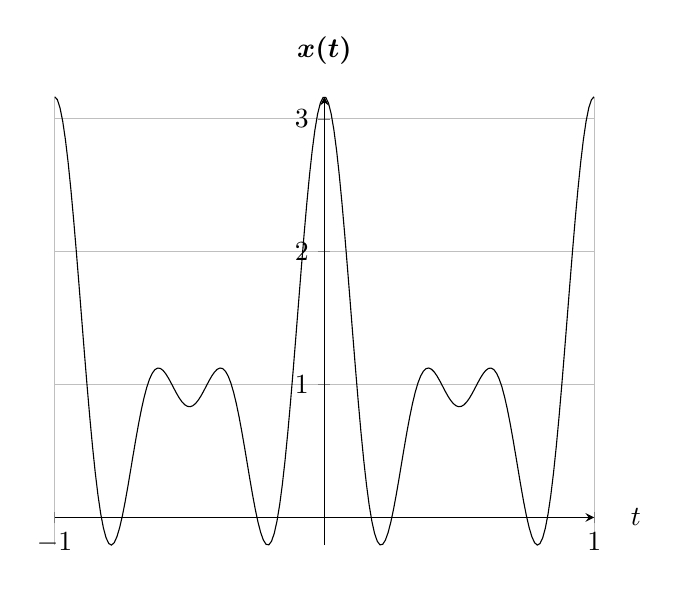
\begin{tikzpicture}[scale=1.0] 
          \begin{axis}[
              axis lines=middle,
              xlabel={$t$},
              ylabel={$\boldsymbol{x(t)}$},
              xtick={-1, 0, 1},
              %ytick={-2, -1, ..., 2},
              %ymin=-2, ymax=2,
              xmin=-1, xmax=1,
              every axis x label/.style={at={(ticklabel* cs:1.05)}, anchor=west,},
              every axis y label/.style={at={(ticklabel* cs:1.05)}, anchor=south,},
              grid,
            ]
            \addplot[domain=-1:1,mark=none,samples=200] {1 + (1/2)*cos(deg(2*pi*x)) + cos(deg(4*pi*x)) + (2/3)*cos(deg(6*pi*x))} node[fill=white, right]{};
          \end{axis}
        \end{tikzpicture}
        \caption{q3a}
        \label{fig:q3a}
    \end{figure}
    
    
    \item %write the solution of q3b
    % TODO: PLOT coefs
    
    \[ x(t) = 1 + \frac{1}{2} cos(2\pi t) + cos(4\pi t) + \frac{2}{3} cos(6\pi t)\]
    
    \[ x(t) = 1 + \frac{e^{j2 \pi t}}{4} + \frac{e^{-j2 \pi t}}{4} + \frac{e^{j4 \pi t}}{2} + \frac{e^{-j4 \pi t}}{2} + \frac{e^{j6 \pi t}}{3} + \frac{e^{-j6 \pi t}}{3}\]
    
    For $\omega_0 = 2\pi$,
    \[a_0 = 1, a_1 = a_{-1} = \frac{1}{4}, a_2 = a_{-2} = \frac{1}{2}, a_3 = a_{-3} = \frac{1}{3}.  \text{ All other } a_k \text{'s } = 0. \]
    
    \begin{figure} [H]
        \centering
        \begin{tikzpicture}[scale=1.0] 
          \begin{axis}[
              axis lines=middle,
              xlabel={$k$},
              ylabel={$\boldsymbol{a_k}$},
              xtick={-4, -3, ..., 4},
              ytick={-1.5, -1, -0.5, ..., 1.5},
              ymin=-1.5, ymax=1.5,
              xmin=-4, xmax=4,
              every axis x label/.style={at={(ticklabel* cs:1.05)}, anchor=west,},
              every axis y label/.style={at={(ticklabel* cs:1.05)}, anchor=south,},
              grid,
            ]
            \addplot [ycomb, black, thick, mark=*] table [x={n}, y={xn}] {q3b.dat};
          \end{axis}
        \end{tikzpicture}
        \caption{q3b}
        \label{fig:q3b}
    \end{figure}
    
    
% TODO: Continue problem
    \item %write the solution of q3c
        ~ \\
        
    \begin{figure} [H]
        \centering
        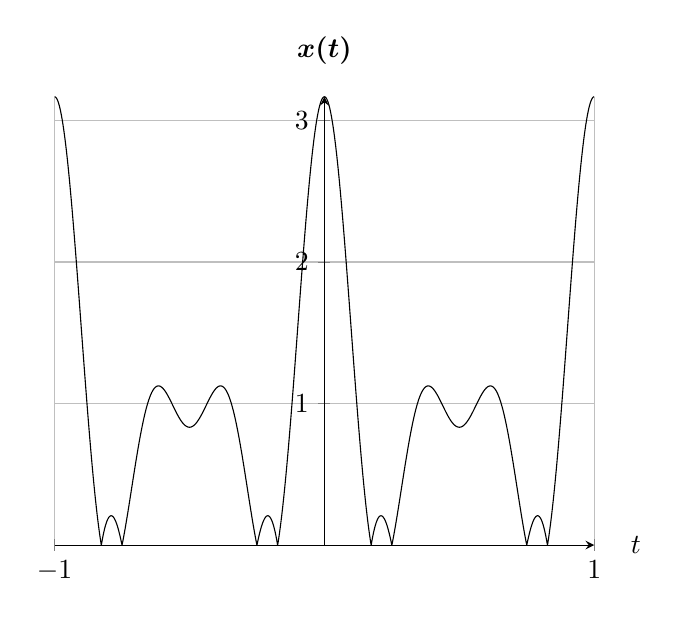
\begin{tikzpicture}[scale=1.0] 
          \begin{axis}[
              axis lines=middle,
              xlabel={$t$},
              ylabel={$\boldsymbol{x(t)}$},
              xtick={-1, 0, 1},
              %ytick={-2, -1, ..., 2},
              %ymin=-2, ymax=2,
              xmin=-1, xmax=1,
              every axis x label/.style={at={(ticklabel* cs:1.05)}, anchor=west,},
              every axis y label/.style={at={(ticklabel* cs:1.05)}, anchor=south,},
              grid,
            ]
            \addplot[domain=-1:1,mark=none,samples=2000] {(1/6) *abs(6 + 3*cos(deg(2*pi*x)) + 6*cos(deg(4*pi*x)) + 4*cos(deg(6*pi*x)))} node[fill=white, right]{};
          \end{axis}
        \end{tikzpicture}
        \caption{Magnitude of q3c}
        \label{fig:q3cm}
    \end{figure}
    
    
    \item %write the solution of q3d
    \end{enumerate}

\item %write the solution of q4
    \begin{enumerate}
    % Write your solutions in the following items.
    % \[ a_k = \frac{1}{T_0} \int_{T_0} x(t) e^{-jk\omega_0 t} \,dt\]
    \item %write the solution of q4a 
    ~\\
    1- Calculating $a_k'$ for $x(t-3)$
    \[ a_k' = \frac{1}{T_0} \int_{T_0} x(t-3) e^{-jk\omega_0 t} \,dt\]
    Substituting $\tau = t - 3$, we obtain
    \[ a_k' = a_k e^{-3jk\omega_0}\]
    
    2- Calculating $a_k''$ for $x(-t)$
    \[ a_k'' = \frac{1}{T_0} \int_{T_0} x(-t) e^{-jk\omega_0 t} \,dt\]
    Substituting $\tau = -t$, we obtain
    \[ a_k'' =  \frac{1}{T_0} \int_{T_0} x(\tau) e^{jk\omega_0 \tau} \,d\tau = -a_k\]
    
    Finally, we combine the results
    \[\frac{a_k'}{3} - \frac{2a_k''}{7} = a_k (\frac{e^{-3jk\omega_0}}{3} + \frac{2}{7})\]
    % Problem 7.7 on https://ocw.mit.edu/resources/res-6-007-signals-and-systems-spring-2011/assignments/
    
    \item %write the solution of q4b
    
    ~\\
    1- 
    Using differentiation property thrice on the function.
    \[ \frac{dx(t)}{dt} \longleftrightarrow (j\omega_0)a_k \]
    
    \[ a_k = (j\omega_0)^3 \cdot a_k \]
    
    
    \end{enumerate}

\item %write the solution of q5
    \begin{enumerate}
    % Write your solutions in the following items.
    \item %write the solution of q5a
    \[ x[n] = sin(\frac{\pi}{2} n)\]
    We choose $\omega_0$ as $2\pi$.Using Euler's relation, we have
    \[ x[n] = \frac{1}{2j} e^{j(\pi/2)n} - \frac{1}{2j} e^{-j(\pi/2)n} \]
    \[ a_0 = 0, a_1 = \frac{1}{2j}, a_{-1} = \frac{-1}{2j} \text{ All other } a_k \text{'s } = 0. \]
    \item %write the solution of q5b
    \[ y[n] = 1 + cos(\frac{\pi}{2} n)\]
    We choose $\omega_0$ as $2\pi$.
    \[ x[n] = 1 + \frac{1}{2} e^{j(\pi/2)n} + \frac{1}{2} e^{-j(\pi/2)n} \]
    \[ a_0 = 1, a_1 = a_{-1} = \frac{1}{2} \text{ All other } a_k \text{'s } = 0. \]
    \item %write the solution of q5c
    Multiplication Property is as follows
    \[ x(t) \longleftrightarrow a_k \text{ and } y(t) \longleftrightarrow b_k \]
    then,
    \[ a_k * b_k \longleftrightarrow \sum_{\forall l} a_l b_{k-l} \]
    
    \[ a_k * b_k \xrightarrow{} a_1 = \frac{1}{2j}, a_{-1} = \frac{-1}{2j}, a_2 = \frac{1}{4j},  a_{-2} = \frac{-1}{4j} \text{ All other } a_k \text{'s } = 0. \]
    
    \item %write the solution of q5d
    \end{enumerate}
    
    \[ z[n] = x[n] * y[n] = \sum_{k=-\infty}^{\infty} x[n - k] \cdot y[k] \]
    \[ z[n] = sin((\pi/2)n) + sin((\pi/2)n)cos((\pi/2)n) \]
    \[ z[n] = sin((\pi/2)n) + \frac{1}{2} sin(\pi n) \]
    We choose $\omega_0$ as $2\pi$. Using Euler's relation, we have
    \[ z[n] = \frac{1}{2j} e^{j(\pi/2)n} - \frac{1}{2j} e^{-j(\pi/2)n} + \frac{1}{4j} e^{j(\pi)n} - \frac{1}{4j} e^{-j(\pi)n} \]
    \[ a_0 = 0, a_1 = \frac{1}{2j}, a_{-1} = \frac{-1}{2j}, a_2 = \frac{1}{4j}, a_{-2} = \frac{-1}{4j} \text{ All other } a_k \text{'s } = 0. \]
    
    Comparing $a_k$ with the $a_k$ from the part (c), we see that both are the same.
    

\item %write the solution of q6

The Fourier series coefficients of $x[n]$, which is periodic with period N, are given by

\[ a_k = \frac{1}{N} \sum_{n=0}^{N-1} x[n] e^{-jk(2\pi / N) n} \]

For $N = 12$,

\[ a_k = \frac{1}{12} \sum_{n=0}^{11} x[n] e^{-jk(\pi / 6) n} \]

\[ a_k = cos(\frac{k\pi}{6}) + sin(\frac{5k\pi}{6})\]
\[ a_k = \frac{1}{2} e^{j(\pi k / 6)} + \frac{1}{2} e^{-j(\pi k / 6)} + \frac{1}{2j} e^{j(5\pi k / 6)} - \frac{1}{2j} e^{j(5\pi k / 6)}\]

Hence,

\[ x[n] = 6 \delta [n-1] + 6 \delta [n-11] - 6j \delta [n-5] + 6j \delta [n-7], 0 \leq n \leq 11 \]

\item %write the solution of q7
    \begin{enumerate}
    % Write your solutions in the following items.

    \item %write the solution of q7a
    \[ x[n] = \sum_{n=0}^{3} a_k e^{jk(2\pi/4) n} \] 
    Period is $N=4$. So the signal $x[n]$ can be expressed as above.
    \[x[0] = a_0 + a_1 + a_2 + a_3 = 0\]
    \[x[1] = a_0 + a_1 e^{j(\pi/2)} + a_2 e^{j\pi} + a_3 e^{j(3\pi/2)} = 1\]
    \[x[2] = a_0 + a_1 e^{j\pi} + a_2 e^{2j\pi} + a_3 e^{j3\pi} = 2\]
    \[x[3] = a_0 + a_1 e^{j(3\pi/2)} + a_2 e^{j3\pi} + a_3 e^{j(9\pi/2)} = 1\]
    The preceding set of linear equations can be reduced to
    \[a_0 + a_1 + a_2 + a_3 = 0\]
    \[a_0 + ja_1 - a_2 - ja_3 = 1\]
    \[a_0 - a_1 + a_2 - a_3 = 2\]
    \[a_0 - ja_1 - a_2 + ja_3 = 1\]
    Solving the equations we get
    \[ a_0 = 1, a_2 = 0, a_1 = a_3 = \frac{-1}{2} \text{ All other } a_k \text{'s } = 0. \]
    % TODO: PLOT
    \begin{figure} [H]
        \centering
        \begin{tikzpicture}[scale=1.0] 
          \begin{axis}[
              axis lines=middle,
              xlabel={$k$},
              ylabel={$\boldsymbol{a_k}$},
              xtick={-3, -2, -1, ..., 3},
              ytick={-3, -2, -1, ..., 3},
              ymin=-3, ymax=3,
              xmin=-3, xmax=3,
              every axis x label/.style={at={(ticklabel* cs:1.05)}, anchor=west,},
              every axis y label/.style={at={(ticklabel* cs:1.05)}, anchor=south,},
              grid,
            ]
            \addplot [ycomb, black, thick, mark=*] table [x={n}, y={xn}] {q7a.dat};
          \end{axis}
        \end{tikzpicture}
        \caption{q7a}
        \label{fig:q7a}
    \end{figure}
    
      
    \item %write the solution of q7b
    
    % TODO: define y[n] in terms of x[n]
    
    \[ y[n] = x[n] - \delta[n + 5] - \delta[n + 1] - \delta[n - 3] - \delta[n - 7] \]
    
    ~ \\
    
    % TODO: PLOT
    \[ y[n] = \sum_{n=0}^{3} a_k e^{jk(2\pi/4) n} \] 
    Period is $N=4$. So the signal $y[n]$ can be expressed as above.
    \[ y[0] = a_0 + a_1 + a_2 + a_3 = 0\]
    \[ y[1] = a_0 + a_1 e^{j(\pi/2)} + a_2 e^{j\pi} + a_3 e^{j(3\pi/2)} = 1\]
    \[ y[2] = a_0 + a_1 e^{j\pi} + a_2 e^{2j\pi} + a_3 e^{j3\pi} = 2\]
    \[ y[3] = a_0 + a_1 e^{j(3\pi/2)} + a_2 e^{j3\pi} + a_3 e^{j(9\pi/2)} = 0\]
    The preceding set of linear equations can be reduced to
    \[a_0 + a_1 + a_2 + a_3 = 0\]
    \[a_0 + ja_1 - a_2 - ja_3 = 1\]
    \[a_0 - a_1 + a_2 - a_3 = 2\]
    \[a_0 - ja_1 - a_2 + ja_3 = 0\]
    Solving the equations we get
    \[ a_0 = \frac{3}{4}, a_2 = \frac{1}{4}, a_1 = \frac{1-2j}{2j} a_3 = \frac{1+2j}{2j} \text{ All other } a_k \text{'s } = 0. \]
    
    
    \begin{figure} [H]
        \centering
        \begin{tikzpicture}[scale=1.0] 
          \begin{axis}[
              axis lines=middle,
              xlabel={$k$},
              ylabel={$\boldsymbol{|a_k|}$},
              xtick={-3, -2, -1, ..., 3},
              ytick={-1, -0.5, ..., 3},
              ymin=-1, ymax=2,
              xmin=-3, xmax=3,
              every axis x label/.style={at={(ticklabel* cs:1.05)}, anchor=west,},
              every axis y label/.style={at={(ticklabel* cs:1.05)}, anchor=south,},
              grid,
            ]
            \addplot [ycomb, black, thick, mark=*] table [x={n}, y={xn}] {q7bm.dat};
          \end{axis}
        \end{tikzpicture}
        \caption{Magnitude of q7b}
        \label{fig:q7bm}
    \end{figure}
    
       
    \begin{figure} [H]
        \centering
        \begin{tikzpicture}[scale=1.0] 
          \begin{axis}[
              axis lines=middle,
              xlabel={$k$},
              ylabel={$\boldsymbol{\phase a_k}$},
              xtick={-3, -2, -1, ..., 3},
              ytick={-1, -0.5, 0, ..., 1},
              ymin=-1, ymax=1,
              xmin=-3, xmax=3,
              every axis x label/.style={at={(ticklabel* cs:1.05)}, anchor=west,},
              every axis y label/.style={at={(ticklabel* cs:1.05)}, anchor=south,},
              grid,
            ]
            \addplot [ycomb, black, thick, mark=*] table [x={n}, y={xn}] {q7bp.dat};
          \end{axis}
        \end{tikzpicture}
        \caption{Phase of q7b}
        \label{fig:q7bp}
    \end{figure}
    
    \end{enumerate}    

\end{enumerate}
\end{document}

